\chapter{Étude des structures de données}


%nombre de caractéristiques ?? de quels type 

%Regarder JDK allocation d'une boite structure


%lister toutes les possibilité - garder toutes les structures - reconstruire l'arbre.. refaire une passe sur le fichier


\section{Introduction}
L'objectif de ce document est de mener une étude sur les différentes structures de données nécessaires aux futurs algorithmes de visualisation. Nous nous intéresserons en particulier à l'opération d'accès à une caractéristique ou d'une donnée d'une boîte ainsi qu'à l'occupation mémoire de cette dernière. Il s'appuie sur le document de spécification (cf : annexe). Ce document sur les calculs de complexité seront réalisés selon le paramètre $n$  représentant le nombre de boîtes, et $d$ est le nombre de dimensions du problème. Le nombre de boîtes réellement utilisées dans le pavage est représenté par $N$. 


\section{Définition de la boîte}
C'est l'entité atomique du pavage. Les accès à ses attributs sont donc cruciaux. On rappelle qu'une boîte est définie de la manière suivante : 
\begin{itemize}
\item 
  Un identifiant : soit des chaînes de caractères (IDStr) respectant un format précis (c.f 1.1 du document de spécifications), soit des entiers positifs (IDInt).
\item
  Une liste de coordonnées dans l'ordre des variables définies en entête. Une liste de type \verb+Interval+.
\item
  Une liste des caractéristiques, dans l'ordre et selon les types définis en entête.
\end{itemize}
Ces données seront régulièrement requises lors de la mise en œuvre des algorithmes nécessaires à la visualisation. Il est donc important que leurs accès soient rapides, voire directs. Pour le cas de l'identifiant, s'agissant d'une simple \verb+String+ le problème de la structure à utiliser ne se pose pas. Pour la liste des coordonnées en revanche, il s'agit d'une séquence finie de données. Plusieurs possibilités sont alors envisageables : 

\begin{itemize}
\item
  Un tableau : L'accès à une coordonnée est direct. Les opérations d'ajout et de suppression sont en revanches coûteuses pour les tableaux dynamiques ($O(n)$).
\item
  Une liste : Si l'accès à une coordonnée n'est pas direct ($O(n)$), les opérations d'ajout et de suppression sont en temps constant.
\item
  Une table de hachage : Coûteuse si la fonction de hachage n'est pas appropriée, une table de hachage propose cependant un accès en $O(1)$.  Cependant le phénomène de collisions (mauvaise répartition des clefs entrainant un conflit entre deux valeurs) est à prendre en considération :

\begin{description}
\item[Implémentation avec un tableau dynamique] Une telle structure permet de garantir un accès en temps constant. Cependant chaque collision va doubler l'occupation mémoire du tableau. Or même si la fonction de hachage est bonne, il est possible d'avoir au moins une collision, ce qui aurait pour conséquence une perte de l'espace mémoire qui se répercuterait sur chaque boîte.
\item[Gestion des collisions avec chaînage] Contrairement à la structure précédente, cette méthode permet de ne pas occuper trop d'espace en chainant les éléments entrants en collision. Malheureusement la complexité en pire cas des opérations d'accès passe en $O(n)$. En revanche, grâce à une bonne fonction de hachage, on accèdera généralement en temps constant sans contre coût mémoire. 
\end{description}

Le passage en revue de ces différentes structures écarte la liste et la table de hachage implémentée par un tableau dynamique. En effet les performances des opérations d'accès de la liste ne sont pas raisonnables. De même l'implémentation d'une table de hachage par un tableau dynamique risque d'entrainer une perte de mémoire trop importante.
%\item
 % Une TreeMap \cite{TreeMap}. Implémentation de base des arbres rouges noirs, cette map a la particularité de posséder des clefs triées. Ainsi les complexités de plusieurs opérations telle que l'accès en $O(\log{n})$. Dans le cas d'un grand nombre de valeurs à stocker, il est plus performant de construire la TreeMap à partir d'une HashMap.

\end{itemize}

%La création d'une boîte a alors une complexité en $O(d)$. De plus l'accès aux différents attributs de la boîte (identifiant, liste des coordonnées) sera en $O(1)$.

\subsection{Généricité des caractéristiques}
Un problème majeur apparaît pour l'instanciation des boîtes. On rappelle qu'une caractéristique à plusieurs types (\verb+String+, \verb+Number+ ou \verb+Interval+). Plusieurs solutions sont envisageables : 
\begin{itemize}
\item
  Une Map unique contenant des \verb+String+ stocke les différentes caractéristiques de la boîte. On aura casté les attributs \verb+Number+ ou \verb+Interval+ en \verb+String+. Il sera alors nécessaire, pour chaque futurs accès, d'effectuer un cast dynamique. On rajoute alors une constante supplémentaire à la complexité de cette opération. 
\item 
Trois tableaux (un pour chaque type) au sein d'une boîte. Trois Maps (une pour chaque type) «générales» au niveau du pavage. La clef d'une map est l'id de la caractéristique et la valeur de la map son indice dans le tableau concret. La boîte peut alors retrouver la valeur de la caractéristique au sein de son tableau.
\item 
  Chaque boîte possède trois Maps pour ces trois types de caractéristiques. 
\end{itemize}


\section{Pavage}
\subsection{Problématique}
%L'outil de visualisation peut charger un fichier entrée de manière dynamique ou non. Nous nous plaçons ici dans le cadre où cette option de chargement dynamique n'est pas activée. \\ 
%L'outil va lire séquentiellement chaque ligne du fichier d'entrée.
Le cahier de spécification exige de l'outil la capacité à charger un pavage de taille non déterminée. Si le nombre de boîtes sera en pratique necessairement borné (limite mémoire de la machine), il faut cependant répondre à cette attente en proposant une structure de stockage capable de supporter un très grand nombre de boîtes. De plus l'outil doit être en mesure de fournir régulièrement des listing spéfiques de boîtes. Par exemple pour afficher la liste de celles concernées par un filtre. La structure du pavage doit être en mesure de répondre de manière efficace à des requêtes de séquences de boîtes selon un ordre particulier. La structure du pavage doit être aussi en mesure de répondre efficacement à la structure  de visualisation graphique (founir rapidement les nouvelles boîtes dans le champs de visualisation, lors d'une rotation de caméra par exemple). Quelles structures de données et quelles stratégies choisir face à de telles exigences ?  %Ce chapitre débute par de le passage en revue de différentes structures de données potentielles. % La création de la structure de stockage débute par la lecture séquentielle du fichier d'entrée (cf section 1  du document de spécification). Plusieurs options apparaissent à cette étape, faut-il par exemple :


%  Le fichier d'entrée est lu une unique fois. Les méthodes de structures dans laquelle les boîtes sont stockées sont suffisamment performantes pour répondre à toutes les spécifications. On peut alors se poser la question s'il faut :


%\begin{enumerate}
 % \item
 %   Insérer les boîtes dans la structure puis la trier plus tard ?
 % \item
 %   Utiliser un tri par insertion ?
%\end{enumerate}


 % Il est possible que refaire des «passes» sur le fichier d'entrée soit une solution. Dans les cas où les opérations de tris et/ou de recherches seraient trop coûteuses pour la structure du pavage (par exemple lors d'une demande de listing de certaines boîtes). On aurait une complexité en pire cas en $O(n)$. 
  % Le création de structure de  données peut alors se faire de différentes  manières : 

\subsection{\'Etude de structures}

\paragraph{Vector :} Collection de données à accès direct par indice. Le nombre de boîte étant donné dans l'entête du fichier d'entrée, une implémenation par un tableau statique proposerait une complexité en $O(n)$ pour l'opération de stockage du pavage. Si l'accès à une boîte à partir de son indice serait direct, l'opération de recherche en revanche aurait une complexité en $O(n)$. 

\paragraph{Dictionnaire :} Collection de données à accès direct par clef. Dans l'hypothèse de posséder une fonction de hachage ne provoquant pas de collisions, une implémentation par une fonction de hachage propose une complexité en $O(n)$ (à nouveau grâce à la connaissance du nombre de boîtes dans l'entête du fichier d'entrée).


%Le nombre potentiellement très grand de boîtes élimine d'emblée la possibilité de choisir une HashMap. En effet même si la fonction de hashage est judicieusement choisie, l'occupation mémoire requise serait bien trop importante. Les listes ne sont pas  appropriées ici. Une complexité en $O(n²)$ pour un accès à une boîte n'est pas raisonnable. Les arbres ont l'atout de pouvoir stocker et manipuler un grand nombre de d'entités. Les arbres de recherches sont des arborescences ordonnées permettant un accès en $O(\log(n))$. Dans le cas où la structure serait triée au fur et à mesure de sa construction. Les arbres de recherche proposent de bonnes performances. Nous développerons pourquoi à travers des cas d'exemples dans les prochains paragraphes : 


\paragraph{Arbre binaire}
Par exemple l'utilisation d'un arbre binaire de recherche pour la création de n boîtes aurait une complexité de $n²$ en pire cas. En effet il s'agit du cas où les boîtes arriveraient triées selon l'ordre inverse de celui que l'on souhaite. Il faudrait alors effectuer $(p-1)$ comparaisons, pour chaque boîte :  $\sum_{p=2}^{n}(p-1)$  Soit $O(n)=\frac{1}{2}n²-\frac{1}{2}n$. Cependant dans le meilleur des cas cette opération a une complexité en $O(n\log{n})$. La création d'un pavage composé de $n$ boîtes à $d$ dimensions aurait alors une complexité égale à: $O(d \times n\log(n))$ 

\begin{figure}[htbp]
  \centering
  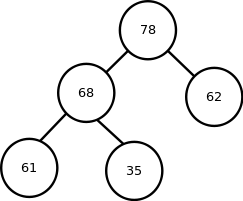
\includegraphics[scale=0.60]{img/binTree}
  \caption{arbre binaire}
  \label{fig:abtree}
\end{figure}
L'arbre binaire était équilibré par définition, la compléxité de son opération de recherche est en $O(log_2 n)$ (hauteur de l'arbre).
   


%http://www.enseignement.polytechnique.fr/profs/informatique/Luc.Maranget/421/poly/arbre-bin.html
\clearpage
\paragraph{Arbres a-b}
Il s'agit d'un arbre de recherche avec les propriétés suivantes :
\begin{itemize}
\item
  $a\leq2$ et $b\leq 2a−1$ deux entiers.
\item
  La racine a au moins 2 fils (sauf si l'arbre ne possède qu'un nœud) et au plus b fils.
  Les feuilles sont de même profondeur.
\item
  Les autres nœuds internes ont au moins a et au plus b fils.
\end{itemize}

\begin{figure}[htbp]
  \centering
  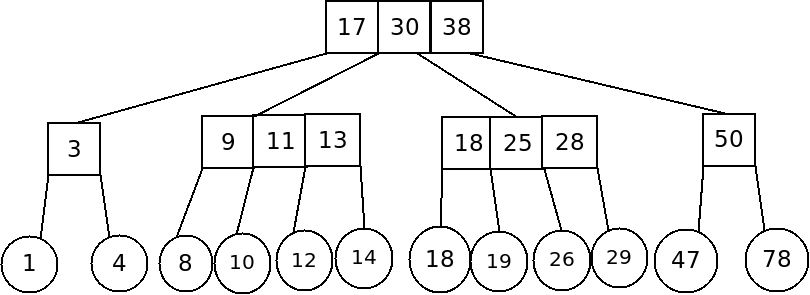
\includegraphics[scale=0.40]{img/abtree}
  \caption{a-b arbre}
  \label{fig:abtree}
\end{figure}

L'avantage des arbres a-b est que leurs hauteurs  sont comprises entres les valeurs suivantes : $ \dfrac{\log{n}}{\log{b}}   \leq h  < 1 + \dfrac{\log{n/2}}{\log{a}}$. Ainsi les opérations d'insertion ne seraient plus en $O(n\log{n})$ mais en $O(\log{n})$. La création d'un pavage composé de $n$ boîtes à $d$ dimensions aurait alors une complexité en $O((n\times d)\log(n))$. La recherche d'un boîte quant à elle aurait une compléxité en $O(\log{n})$.

